\section{Styrning av robot}
\subsection{Start av Mjukvara}
\begin{enumerate}
	\item Om anslutning har etablerats till Gloria så behöver man hitta filen mainThread.py som ligger i home directory, dvs där man hamnar när man väl har ssh:at in (se Användning av Systemet).
	\item Kommandot för att starta systemet i Gloria är bara en rad: python mainThread.py
	När detta kommandot körs så sätter systemet igång och Gloria lägger sig i vänteläge.
	\item Efter att mainThread.py har startats på Gloria så startar man upp en ny terminal lokalt på datorn som Gloria ska styras ifrån och hittar Gui.py. Sedan kör man kommandot: python Gui.py
	\item Anslut två joysticks via USB (till pc). Klargör vilken som styr motor och vilken som styr arm.
\end{enumerate}
\subsection{Användning av Mjukvara}
\begin{enumerate}
	\item Styrning av Gloria sker som följer: 
	\begin{itemize}
		\item Väl inne i Gui.py, tryck på \textbf{connect arm joystick} för att ansluta joysticken som styr armen.
		\item Samma procedur gäller för joysticken som styr motorn.
		\item Ange Glorias statiska IP-adress (192.168.99.1) i connect-fältet och tryck på \textbf{connect}.
		\item Motor: Joystick 1 låter användaren köra i alla riktningar. Framåt-tilt får Gloria att accelerera framåt, bakåt-tilt ger samma effekt bakåt. Vänster orsakar en vänstersväng (vänster hjulpar kör långsammare än höger) och höger fungerar på samma sätt.
		\item Arm: Armen (Gripklon) styrs i ett 3D-rum utifrån hur man rör Joystick 2 där gripklon är koordinaten i planet. Rörelserna beräknas automatiskt, så dessa behöver användaren inte ta hänsyn till. 
		\item Gripklo framåt/bakåt/vänster/höger: Tilta Joysticken i önskad rikting.
		\item Höj/Sänk Gripklon: %todo
		\item Rotera vristen: Vrid Joysticken åt vänster/höger
		\item Gripklo (släpp, grepp): Höger pedal på baksida av Joysticken regleras från 0 till 1, där 0 innebär att gripklon är helt öppen och 1 innebär att den är stängd.
		
	\end{itemize}
	\item Knapparna i nedre vänstra hörnet på GUI gör följande:
	\begin{itemize}
		\item start: Startar Glorias mainloop, behöver göras innan några andra kommandon kan accepteras.
		\item calibrate tape: Kalibrerar sensorvärdet för tejp.
		\item calibrate floor: Kalibrerar sensorvärdet för golv.
		\item got package: Signalerar till Gloria att man är klar med att plocka upp ett packet med Joysticken.
		\item auto motor: Sätter motorerna i autonomt läge, vilket får Gloria att köra av sig själv givet sensordata.
		\item auto arm: Sätter armen i autonomt läge.
	\end{itemize}
	\begin{figure}[h]
	\center
	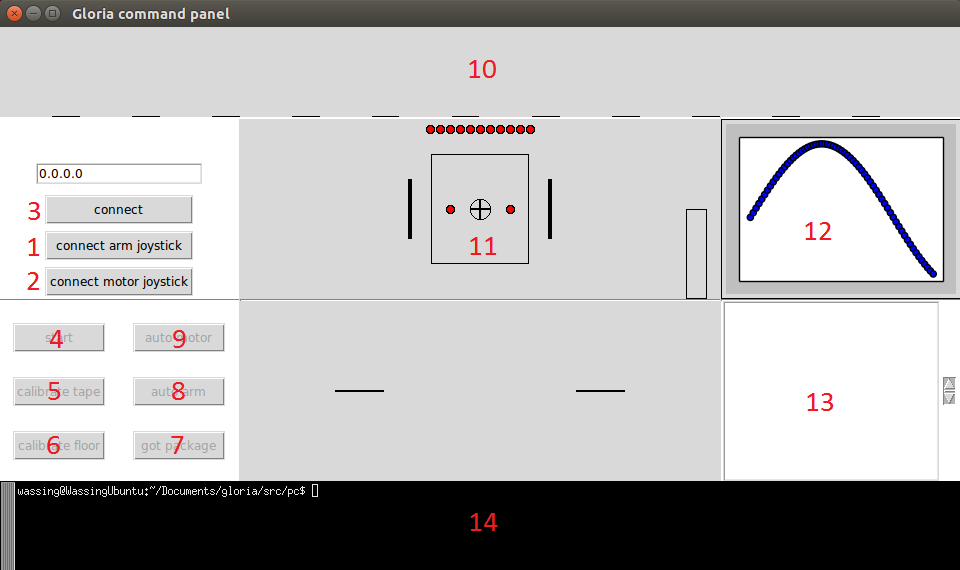
\includegraphics[scale=0.6]{Gui.png}
	\endcenter
	\caption{Gui. Överst visas sensordata, i mitten visas gloria, till vänster alla relevanta knappar, till höger visas reglerfel samt errorcodes och nederst visas en terminal.}
	\end{figure}
\end{enumerate}